% 2D differential element with stresses and body forces
\begin{tikzpicture}[scale=1.0,font=\small]
  \def\a{3.0}
  \draw[thick] (0,0) rectangle (\a,\a);
  \node[anchor=north west,inner sep=2pt] at (0,\a*0.55) {$dy$};
  \node[anchor=south west,inner sep=2pt] at (\a*0.55,0) {$dx$};
  % body forces
  \draw[->] (\a/2,\a/2) -- ++(0.8,0) node[below] {$f_x$};
  \draw[->] (\a/2,\a/2) -- ++(0,0.8) node[right] {$f_y$};
  % left face
  \draw[->] (0,\a/2) -- ++(-1.1,0) node[left] {$\sigma_{xx}$};
  \draw[->] (-0.45,\a-0.2) -- (-0.45,0.2);
  \node[left] at (-0.5,0.55) {$\sigma_{xy}$};
  % right face
  \draw[->] (\a,\a/2) -- ++(1.1,0) node[right] {$\sigma_{xx}+\dfrac{\partial\sigma_{xx}}{\partial x}dx$};
  \draw[->] (\a+0.45,0.2) -- (\a+0.45,\a-0.2);
  \node[anchor=north west] at (\a+0.3,-0.1) {$\sigma_{xy}+\dfrac{\partial\sigma_{xy}}{\partial x}dx$};
  % bottom face
  \draw[->] (\a/2,0) -- ++(0,-1.2) node[right] {$\sigma_{yy}$};
  \draw[->] (\a-0.2,-0.45) -- (0.2,-0.45);
  \node[below] at (0.7,-0.5) {$\sigma_{xy}$};
  % top face
  \draw[->] (\a/2,\a) -- ++(0,1.3) node[above] {$\sigma_{yy}+\dfrac{\partial\sigma_{yy}}{\partial y}dy$};
  \draw[->] (0.2,\a+0.45) -- (\a-0.2,\a+0.45);
  \node[anchor=south east] at (\a*0.3,\a+0.5) {$\sigma_{xy}+\dfrac{\partial\sigma_{xy}}{\partial y}dy$};
\end{tikzpicture}
